\Needspace{10\baselineskip}
\section{CNN 推理协处理器}
\label{sec:cop}
协处理器执行紧固件分类网络的 INT8 推理，数据通路与寄存器接口见图~\ref{fig:cop}。
整数语义由 C02 契约冻结（表~\ref{tab:c02}），集成分工由 C03 契约冻结。

\begin{figure}[H]\centering
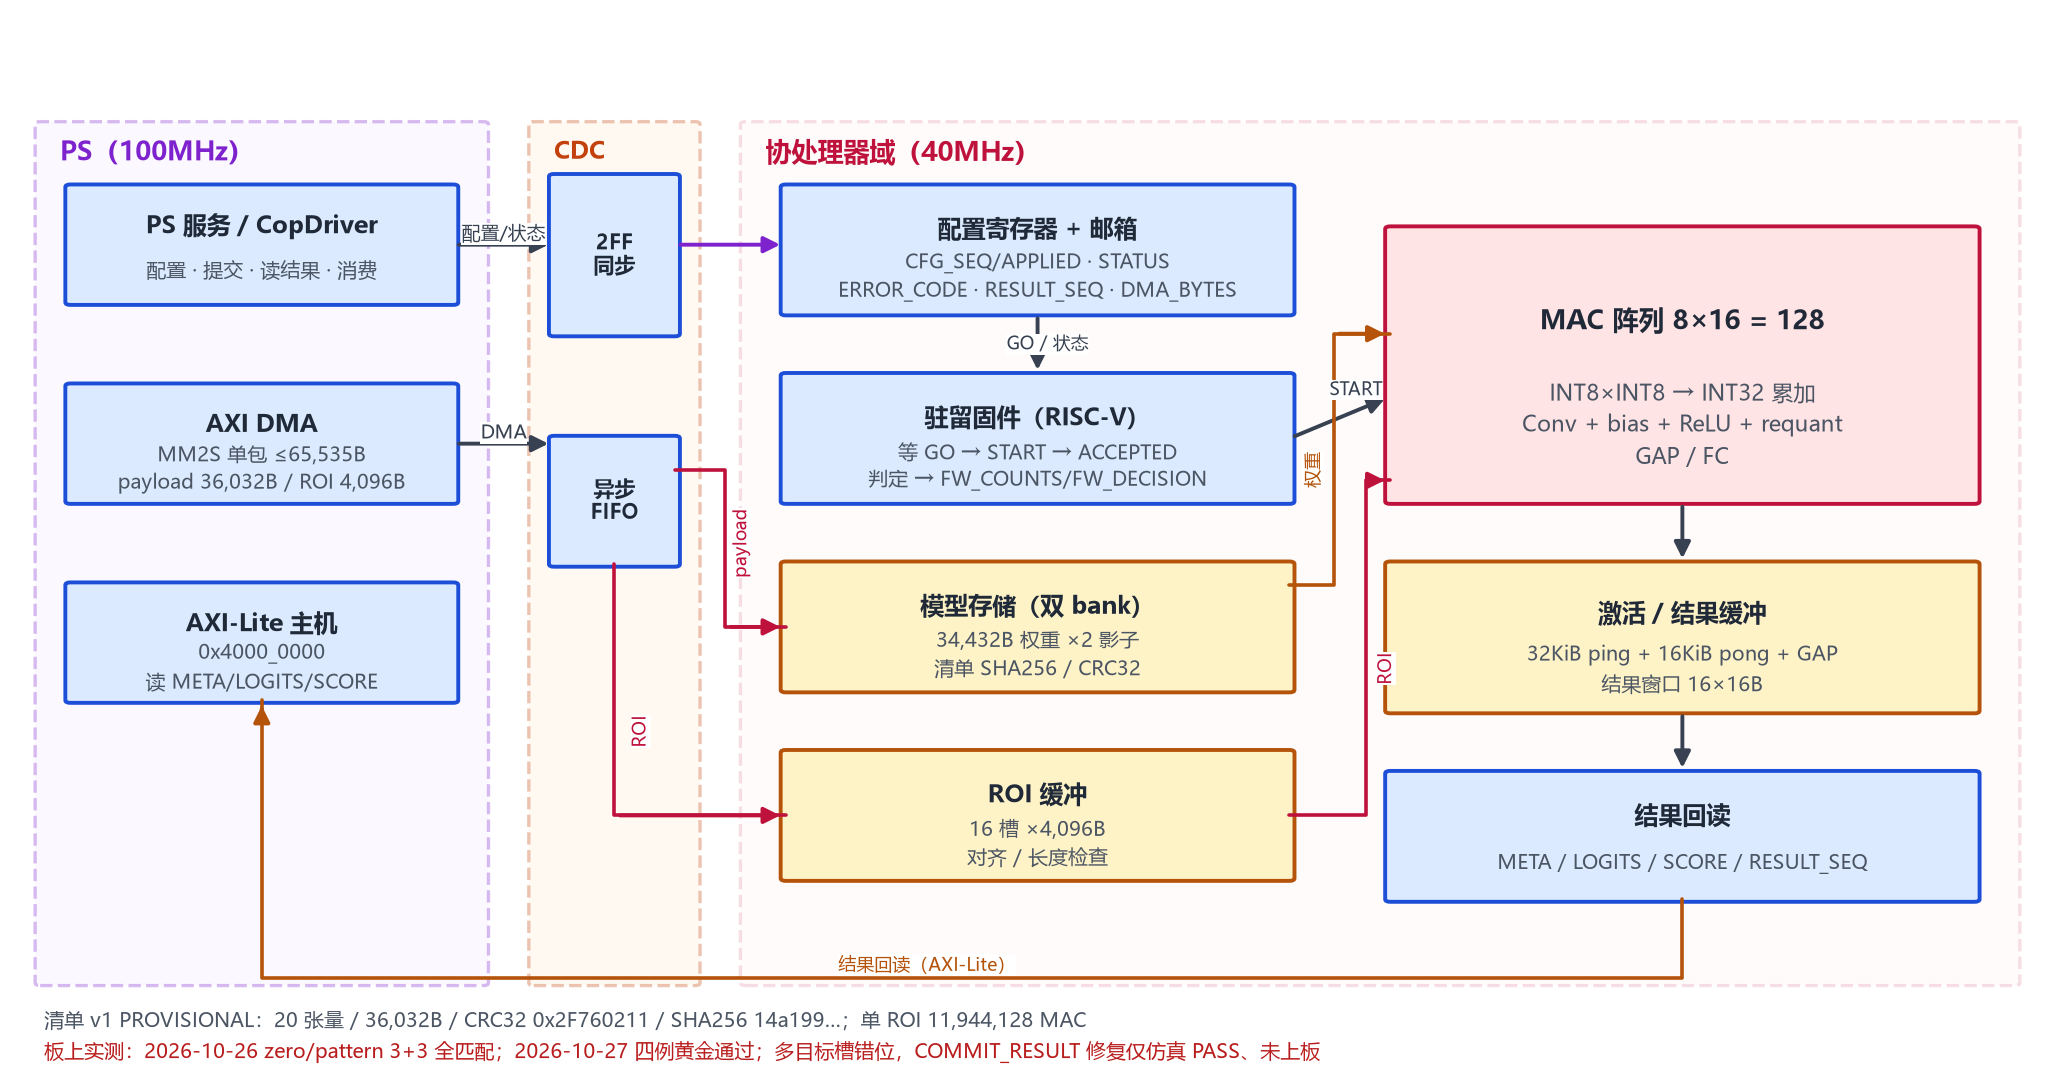
\includegraphics[width=0.98\linewidth]{fig_cop.png}
\caption{CNN 协处理器数据通路、寄存器与 DMA（仓库配图）}\label{fig:cop}
\end{figure}

\begin{table}[H]\centering\small
\caption{C02 整数契约要点}\label{tab:c02}
\begin{tabularx}{\linewidth}{@{}P{34mm}Y@{}}\toprule
项目 & 约定\\\midrule
输入 & 64$\times$64 灰度 ROI\\
权重量化 & per-channel 对称 INT8\\
激活量化 & per-tensor INT8\\
累加 & INT32\\
再量化 & multiplier + 右移 + 饱和\\
计算阵列 & 128 MAC（8$\times$16），100 MHz\\
结果语义 & 并列时取较小类别；\code{score_q15} 线性映射裕度\\\bottomrule
\end{tabularx}\end{table}

\subsection{微架构与优化}
整网控制器调度卷积、偏置、ReLU、再量化、全局平均池化与全连接。
初版综合 WNS $-19.892$ ns，经分拍重整后收敛至 +0.058 ns（192 DSP）。
快速模式重排发射调度后：整网 1{,}123{,}109 拍降至 472{,}593 拍，DSP 192$\rightarrow$136，LUT 10{,}100$\rightarrow$4{,}540。
权重存储采用 16 路 64-bit bank 的真实读延迟 BRAM，每发射拍 136 字节；容量与端口带宽分别核算，不以容量替代端口验证。

\subsection{生产与消费握手}
任务握手语义：PS 独占 \code{CONSUME} 清终态；\code{ACCEPTED} 粘滞；\code{RESULT_SEQ} 单调递增。
固件按\emph{校验序号、落盘成功、再消费}的顺序处理，宁可停顿不以丢数据换流畅。
固件 \code{cop_job.c} 为 52 行 RV32I 代码，与主机共用判定头文件。
看门狗覆盖 \code{NO_ACK}、硬件超时与过期结果三类异常。

\subsection{板级集成与门禁}
板级集成的关键决策：
DMA 描述符长度位宽由 14 位扩至 16 位，36{,}032 字节负载单笔传输，禁止分包（每笔 DMA 产生 TLAST）；
加载器 fail-closed，manifest、SHA256、CRC32 与 HWH 四重校验不过即拒绝；
IMEM 初值设四重门禁（绝对路径、首字校验、RAMB INIT 回读、综合日志扫描），杜绝位流不带固件的假通过；
时钟采用片内 MMCM 产生 40 MHz 并由 HWH 绑定核对，PS 直供方案曾被时钟门禁拦截（实测 142.857 MHz）。
整机门禁的演进见表~\ref{tab:wholegate}。
整机（非 OOC）门禁断言 WNS$\geq$0、DSP$\leq$220、BRAM36$\leq$140、check\_timing 四项为零、DRC 为零、锁存器为零、CDC 例外清单 fail-closed；部件 OOC 资源相加不得冒充整机结果。

\begin{table}[H]\centering\small
\caption{整机门禁演进（40 MHz 整机构建）}\label{tab:wholegate}
\begin{tabularx}{\linewidth}{@{}P{34mm}P{30mm}Y@{}}\toprule
构建 & WNS & 说明\\\midrule
2026-10-22 首过 & +2.498 ns & 修复资源超限与未约束端点后\\
2026-10-26 边沿修复版 & +3.062 ns & DSP 136、BRAM36 69\\
2026-10-27 A 包 & +2.078 ns & 116/116 文件校验，随核共存\\\bottomrule
\end{tabularx}\end{table}

\subsection{板上验证}
2026-10-26，协处理器首次获得实板硬件 CNN 输出：zero 与 pattern 诊断网各 3 轮，6/6 与预期一致。
随后四例黄金（zero、pattern、\code{roi_001}、frame）全部匹配，寄存器 10{,}000 次连续读取无错误。
共存位流同时输出 HDMI、抓取 BGR 原帧并运行硬件 CNN。
2026-10-28，多目标修复包上板：CNN r6 两组真实 ROI 共 12 轮 85 个结果，logits、类别、有效位与裕度同整数参考逐项一致，结果槽错位未再出现（WNS 1.359 ns 位流）。
以上为单目标与多目标推理正确性证据；识别精度见第~\ref{sec:data} 节的边界说明。
\FloatBarrier
